%%%%%%%%%%%%%%%%%%%%%%%%%%%%%%%%%%%%%%%%%%%%%%%%%%%%%%%%%%%%%%%%%%%%%%%%%%%%%%%
% Neuroimage-like layout
\documentclass[5p]{elsarticle}
% For kindle
%\documentclass[1p,12pt]{elsarticle}
%\usepackage{geometry}
%\geometry{a6paper,hmargin={.2cm,.2cm},vmargin={1cm,1cm}}
% End kindle
\usepackage{graphicx}
\usepackage{amsmath,amsfonts,amssymb}
\usepackage{xfrac}
\usepackage{bm}
\usepackage{algorithm}
\usepackage{algorithmic}
\usepackage{afterpage}
\usepackage{url}
\usepackage[breaklinks=true,letterpaper=true,colorlinks,bookmarks=false]{hyperref}
\usepackage[table]{xcolor}
\usepackage{booktabs}  % For toprule
\usepackage{multirow}
%\usepackage{stfloats} % To have double-column floats at the bottom
% (without this, it {figure*}[b] is impossible

% Never place a float before its reference
%\usepackage{flafter}

% For review: line numbers
%\usepackage[pagewise]{lineno}
\usepackage[switch]{lineno}
\modulolinenumbers[5]


\bibliographystyle{model2-names.bst}\biboptions{authoryear}


\definecolor{deep_blue}{rgb}{0,.2,.5}
\definecolor{dark_blue}{rgb}{0,.15,.5}

\hypersetup{pdftex,  % needed for pdflatex
  breaklinks=true,  % so long urls are correctly broken across lines
  colorlinks=true,
  linkcolor=dark_blue,
  citecolor=deep_blue,
}

% Float parameters, for more full pages.
\renewcommand{\topfraction}{0.9}	% max fraction of floats at top
\renewcommand{\bottomfraction}{0.8}	% max fraction of floats at bottom
\renewcommand{\textfraction}{0.07}	% allow minimal text w. figs
%   Parameters for FLOAT pages (not text pages):
\renewcommand{\floatpagefraction}{0.6}	% require fuller float pages
%    % N.B.: floatpagefraction MUST be less than topfraction !!
\renewcommand{\dbltopfraction}{.95}  % double page floats at the top
\renewcommand{\dblfloatpagefraction}{.6}
\setcounter{totalnumber}{4}
\setcounter{topnumber}{3}
\setcounter{dbltopnumber}{3}
\setcounter{bottomnumber}{2}

\def\B#1{\mathbf{#1}}
%\def\B#1{\bm{#1}}
\def\trans{^\mathsf{T}}
% A compact fraction
\def\slantfrac#1#2{\kern.1em^{#1}\kern-.1em/\kern-.1em_{#2}}
\newlength{\mylength}%

%%%%%%%%%%%%%%%%%%%%%%%%%%%%%%%%%%%%%%%%%%%%%%%%%%%%%%%%%%%%%%%%%%%%%%%%%%%%%%
% For the final version: to output PDF figures from latex
\newif\iffinal
\finaltrue
%\finalfalse
\iffinal\else
\usepackage[tightpage,active]{preview}
\fi

%%%%%%%%%%%%%%%%%%%%%%%%%%%%%%%%%%%%%%%%%%%%%%%%%%%%%%%%%%%%%%%%%%%%%%%%%%%%%%
% Modification tracking
\usepackage{xcolor}
\usepackage[normalem]{ulem}
\colorlet{markercolor}{purple!50!black}
\newcommand{\ADDED}[1]{\textcolor{markercolor}{\uline{#1}}}
\newcommand{\DELETED}[1]{\textcolor{red}{\sout{#1}}}

% For highlighting changes for reviewer
\usepackage{MnSymbol}
\def\marker{%
    \vadjust{{%
	\llap{\smash{%
	    \color{purple}%
	    \scalebox{1.8}{$\filledmedtriangleright$}}\;}%
    }}\hspace*{-.1ex}%
}%
\def\hl#1{\textcolor{markercolor}{%
   \protect\marker%
  #1%
}}%


% Show the old version
%\renewcommand{\ADDED}[1]{}
%\renewcommand{\DELETED}[1]{#1}

% Show the new version
%\renewcommand{\ADDED}[1]{#1}
%\renewcommand{\DELETED}[1]{}

%%%%%%%%%%%%%%%%%%%%%%%%%%%%%%%%%%%%%%%%%%%%%%%%%%%%%%%%%%%%%%%%%%%%%%%%%%%%%%%%
\begin{document}
% Show line numbers
%\linenumbers
%\linenumbersep 3pt\relax
%\renewcommand\linenumberfont{\normalfont\tiny\sffamily\color{black!50}}

\journal{NeuroImage}
\title{Towards a better predictive model of rest fMRI: benchmarks across
multiple phenotypes}


%\author[parietal,cea]{Ga\"el Varoquaux\corref{corresponding}}
\author[parietal,cea]{Kamalaker Dadi}

\cortext[corresponding]{Corresponding author}

\address[parietal]{Parietal project-team, INRIA Saclay-\^ile de France,
France}
\address[cea]{CEA/Neurospin b\^at 145, 91191 Gif-Sur-Yvette, France}


\begin{abstract}
%
%
\end{abstract}

\begin{keyword}
    rs-fMRI; functional connectivity; predictive modeling; phenotypes;
    classification
\end{keyword}

\maketitle%

%%%%%%%%%%%%%%%%%%%%%%%%%%%%%%%%%%%%%%%%%%%%%%%%%%%%%%%%%%%%%%%%%%%%%%%%%%%%%%%%
%\smash{\raisebox{20em}{{\sffamily\bfseries Comments and Controversies}}}%
\vspace*{-3em}%

\sloppy % Fed up with messed-up line breaks

% XXX: read other commentary paper, for instance the Frison one
% Q: how much should I be citing things

\section{Introduction}%

% Start positive

% Introduce cross-validation
% State the problem
% Explain what I do, and our conclusion

% XXX: TODO: announce the content of the paper

\section{Methods}

\subsection{Overview of the pipeline}
\autoref{fig:pipeline}  depicts  our  prediction  pipeline.  It  consists  of  four
steps: i) Definition  of  brain  regions  of  interest  (ROIs),
ii) Extraction  of  the  time  series  associated  with  these  ROIs,
iii) Estimation  of  FC  metrics  from  these  time  series,
iv) Connectivity-based classification of the phenotypic target.
\subsection{Definition of brain regions or networks}

\subsection{Parameterizing connectivity}

\subsection{Supervised learning: Classifiers}

\section{Experimental study}

\subsection{rs-fMRI Datasets}

\subsection{Data \& prediction task}
\subsection{Cross validation}


%\paragraph{Previous results: cross-validation on brain images}


\begin{figure*}[t]
    \setlength{\fboxsep}{0pt}%
    \begin{minipage}[T]{.26\paperwidth}
     \includegraphics[height=.28\paperwidth]{pipeline.pdf}%
     \llap{\raisebox{.265\paperwidth}{%
	\parbox{.28\paperwidth}{\colorbox{white}{\bfseries\sffamily
	\hspace*{-.15ex}\,\hspace{-2ex}}}}}%
    \medskip
    \end{minipage}
    \caption{\textbf{Resting-state functional connectivity prediction pipeline}}

    {\bfseries\sffamily 1} -- Defining Brain ROIs: involves using three
    pre-defined atlases - Automated Anatomical Labeling (AAL) - Harvard Oxford
    - Bootstrap Analysis of Stable Clusters (BASC) and using four data-driven
    methods - Linear decomposition models: Group Independent Component
    Analysis (Group ICA) - Online Dictionary Learning (DictLearn) and
    Clustering models: KMeans - Agglomerative with Ward criterion. For each
    data-driven method, we build the atlas on training data ($75\%$) on each
    split (n=100) and use this atlas for the consecutive step. 
    %
    {\bfseries\sffamily 2} -- Timeseries signal extraction: For each atlas or
    ROIs, from Step 1 are used in extracting subject specific timeseries signals.
    %
    {\bfseries\sffamily 3} -- Parameterizing functional connectivity between
    ROIs,  using  correlation,  partial  correlation  or  tangent  space
    embedding
    %
    {\bfseries\sffamily 4} -- Supervised learning: Classifiers, a classification
    model is built to predict groups with two linear classifiers, SVC ($\ell_{1}$ or
    $\ell_{2}$ penalization) and ridge regression ($\ell_{2}$ penalization).
    %
    Cross-validation for 100 splits with $75\%$ training set and remaining
    $25\%$ test is used in Step 4, classification setting and reported scores
    are Receiver Operating Characteristic and Area Under the Curve (ROC-AUC)
    \label{fig:pipeline}
\end{figure*}


%\paragraph{Spread out predictions in a public challenge}

%website\footnote{\url{https://www.kaggle.com/c/mlsp-2014-mri}}.
\section{Results}

%    \begin{tabular}{llccl}
%    \toprule
%    Dataset        &       atlas &          classifier &    measure &
%    Score \\
%	%strategy  &        size &    error bar &    error bar \\
%    \toprule
%    \multirow{8}{9ex}{ADNI} & AAL &  SVC{$\ell_{1}$} &  correlation & $0.64$ \\
%                            &           BASC &  Ridge &   Tangent &    $0.71$ \\
%                            & DictLearn &  SVC{$\ell_{2}$} &   Tangent & $0.75$ \\
%                        &          Harvard Oxford &  Ridge & Tangent &   $0.66$ \\
%                            & Group ICA & Ridge & Tangent & $0.75$ \\
%                  & KMeans & Ridge & Tangent & $0.75$ \\
%                 & Ward & Ridge & Tangent & $0.71$ \\
%    \midrule                                            
%    \multirow{8}{9ex}{} & 30 &   &  \\
%                  &         100 &   &    \\
%                  &         300 &   &    \\
%	          &        1000 &   &    \\
%    \bottomrule
%    \end{tabular}}
%
%    \centering
%    \caption{\textbf{Comparison of the atlas impact on prediction accuracy.}
%        Reported values are the mean of AUC over 100 iterations.
%        Best predictions are in bold.}
%     \label{tab:accuracy}
%     \begin{tabular}{ccccc}
%         & COBRE & ADNI & ACPI & ADNIDOD \\
%         \hline\\[-2mm]
%         AAL       & $.81$ & $.64$ & $.55$ & $\bf .71$ \\
%         BASC      & $.82$ & $0.71$ & $0.56$ & $0.67$ \\
%         DictLearn & $\bf{ 0.85}$ & $\bf 0.75$  & $\bf 0.57$ & $\bf 0.68$ \\
%         HO        & $0.72$ & $0.66$ & $0.57$ & $0.65$ \\
%         ICA       & $0.83$ & $\bf 0.75$ & $0.55$ & $0.67$ \\
%         K-Means   & $0.84$ & $\bf 0.75$ & $\bf 0.58$ & $0.68$ \\
%         Ward      & $0.84$ & $0.71$ & $0.55$ & $\bf 0.69$ \\
%     \end{tabular}
% \end{table}
 \subsection{Choice of classifier}

\begin{figure}
    \centerline{%
    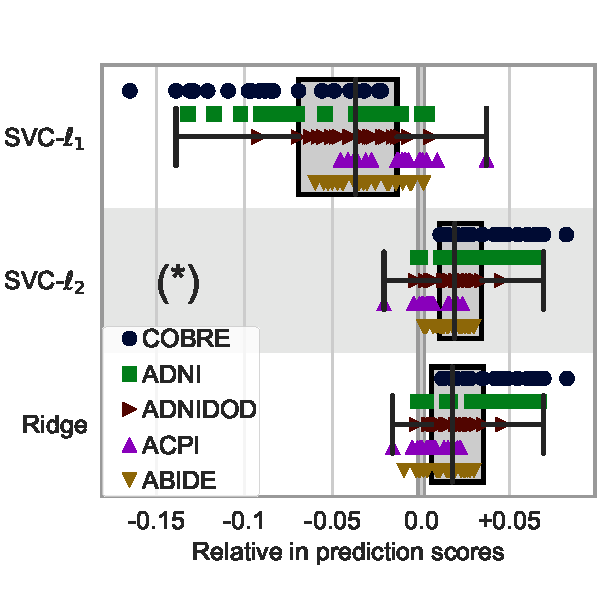
\includegraphics[width=.8\linewidth]{impact_plot_classifier.pdf}%
    }%
    \caption[choice of classifier]{\textbf{Impact of classifier choices on
    prediction scores}
\label{fig:impact_classifier}}
\end{figure}

\subsection{Choice of connectivity parameterization}


\begin{figure}
    \centerline{%
    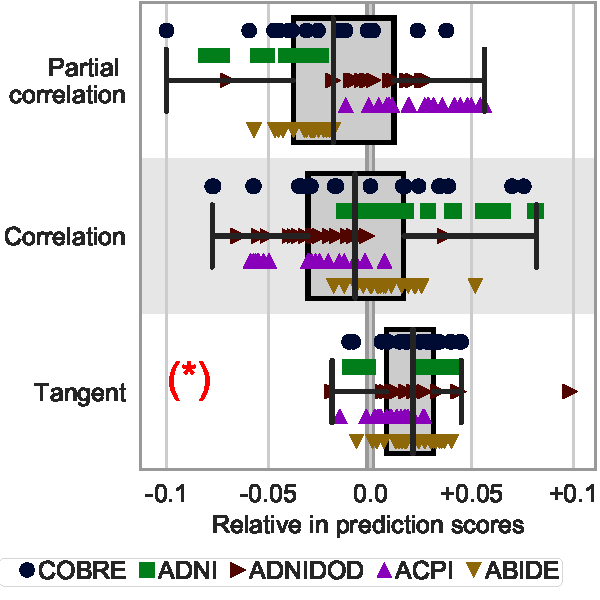
\includegraphics[width=\linewidth]{impact_plot_measure.pdf}%
    }%
    \caption[choice of classifier]{\textbf{Impact of connectivity
            parameterization method choices on prediction scores}
\label{fig:impact_connectivity}}
\end{figure}

\subsection{Choice of atlas methods: Either regions or networks}

\begin{figure}
    \centerline{%
    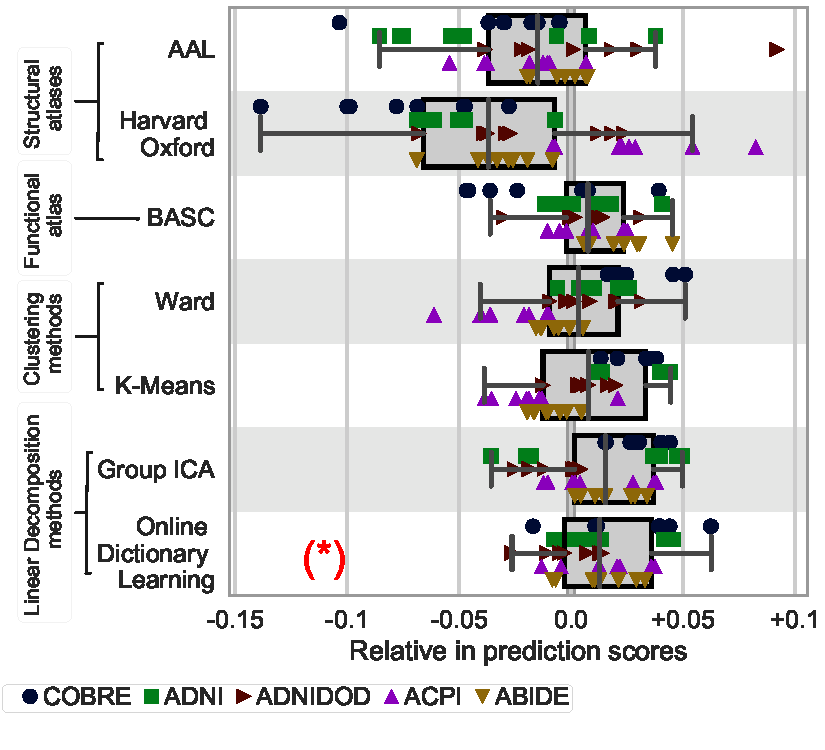
\includegraphics[width=\linewidth]{impact_plot_atlas.pdf}%
    }%
    \caption[choice of atlas]{\textbf{Impact of atlas choices
        on prediction scores}
    \label{fig:impact_atlas}}
\end{figure}

\paragraph{Effect of dimensionality: Brain regions}

\begin{figure}
    \centerline{%
	\includegraphics[width=\linewidth]{dot_plot_n_regions_suppressed_background.pdf}%
    }%
    \caption[]{\textbf{Effect of dimensionality: Choice of brain regions} {For
            each of four atlases (ICA, DictLearn, KMeans, BASC) driven with region
            extraction, we show the measure of effect on prediction scores obtained by
            removing the mean effect of group relatively over all
            cross-validation splits and datasets.

            What we obtain then, is the demeaned score for each split and for each
            dataset.

            Given that, we plot here: for each atlas, we took the average of
            calculated demeaned scores over all splits which is showed on y-axis
            as choice of vary in dimensionality as showed on x-axis.
            
            For each atlas, we then see the effect of each dataset (each unique color)
            by projecting an error bar plot with $95\%$ confidence interval on each
            averaged score shown as violin plot in gray color.
            
            Given the plots, we choose here the best dimensionality in ICA of
            $80$, and DictLearn of $60$, KMeans of $120$ and BASC of $122$.
        
            These references in finding an optimalilty dimensionalities are
            then used for further comparisons of choosing the best atlas
            method.}
    %
    \label{fig:effect_size_in_regions}
    }
\end{figure}


To understand better the choice of atlas defined with or without region
extraction as a function of vary in dimensionality, we chose to see the mean
effect on prediction scores overall the cross validation folds with respect to
four reference atlases (ICA, Dictionary Learning, KMeans and BASC) with
various dimensionalities. \autoref{fig:effect_size_in_regions} outlines to choose
between the optimal dimensionality for each atlas as a function of regions.

\paragraph{Effect of dimensionality: Brain networks/parcellations}
%
\begin{figure}
    \centerline{%
	\includegraphics[width=\linewidth]{dot_plot_parcellations_suppressed_background2.pdf}%
    }%
    \caption[]{\textbf{Effect of dimensionality: Choice of brain
        networks/parcellations} {Atlases based on networks: ICA, DictLearn,
            BASC whereas based on parcellations are KMeans and Ward. In total,
            we are comparing here five brain atlases each driven without
            region extraction.

            We show the measure of effect on prediction scores obtained by
            removing the mean effect of group relatively over all cross-validation
            splits and datasets.

            As demonstrated in \autoref{fig:effect_size_in_regions}, we show
            the same the demeaned score for each split and for each dataset
            but this time without region extraction.

            Given that, we plot here: for each atlas, we took the average of
            calculated demeaned scores over all splits which is showed on y-axis
            as choice of vary in dimensionality as showed on x-axis.
            
            For each atlas, we then see the effect of each dataset (each unique color)
            by projecting an error bar plot with $95\%$ confidence interval on each
            averaged score shown as violin plot in gray color.
            
            Given the plots, we choose here the best dimensionality in
            networks: ICA of $80$, and DictLearn of $60$, KMeans of $120$ and BASC
            of $122$ and Ward of $120$.
        
            These references in finding an optimalilty dimensionalities without
            region extraction are then used for further comparisons of choosing
            the best atlas method.}
    %
    \label{fig:effect_size_in_networks}
    }
\end{figure}

\paragraph{Which is better: Brain atlases with regions or without regions}
Given the outlining the choice of optimal dimensionality of brain atlases with
or without regions extracted as shown in \autoref{fig:effect_size_in_regions}
and \autoref{fig:effect_size_in_networks}, we compare them to see which is
better in prediction. Prediction using atlases build with regions or
using atlases build with networks. As shown in
\autoref{fig:regions_vs_nonregions}, and atlas GroupICA or ICA, predicting
using regions is better rather than using only networks. Whereas for
Dictionary Learning, prediction using regions is better and same even with
BASC atlases. Interesting, to see that BASC which is a pre-defined atlase
built on unseen resting state functional datasets is better with regions
rather than only networks. While we see the opposite with KMeans based atlas
prediction. With KMeans, using parcellations without regions or
inter-hemispheric separation is better for prediction tasks of resting state
fMRI.

\begin{figure}
    \centerline{%
	\includegraphics[width=\linewidth]{violin_plot_mean_score_region_extraction_ica_dict_kmeans.pdf}%
    }%
    \caption[regions vs non regions]{\textbf{Which is better for prediction: regions or
        without regions}
        For each atlas (ICA, DictLearn, KMeans and BASC), we show here the
        best setting for prediction by measuring its impact on prediction
        accuracy for each dataset.

        Each data point is a measure of impact on prediction accuracy. For
        each atlas, data point in unique color is a score obtained by averaging
        raw prediction scores grouped by three classifiers, three measures.
        Each unique color is referred to each of four datasets used to test
        the prediction. 

        We then compare these data points using violin plots with or without
        region extraction. On x-axis is the impact on prediction and on y-axis
        is to differentiate between region extraction and no region extraction.

        From the observations, ICA atlas based prediction has better impact
        by extracting regions on the networks which is quite similarly
        observed with Online Dictionary Learning and BASC. But, KMeans has
        better impact when predicted using without region extraction meaning
        that parcellations based atlas.
    %
    \label{fig:regions_vs_nonregions}
    }
\end{figure}

\section{Supplementary material}

\begin{figure}
    \centerline{%
	\includegraphics[width=.8\linewidth]{n_regions_vs_dimensionality.pdf}%
    }%
    \caption{\textbf{Number of regions extracted with dimensionality}
    %
    %
    \label{fig:n_regions_dim}
    }
\end{figure}

\begin{table}[t]
    \begin{tabular}{llllrlll}
        \toprule
        & Atlas &    Classifier & Measure &  Dimensionality & Regions & 
        ROC\textunderscore AUC &  Dataset \\
        \midrule
        &  Online Dictionary Learning & SVC-$\ell{_2}$ & Tangent & 60 & yes &
        0.86\$\textbackslashpm\$0.06 &    COBRE \\
        & K-Means & Ridge & Tangent & 120 & no &
        0.76\$\textbackslashpm\$0.09 &
        ADNI \\
        &                            AAL &  SVM-\$\textbackslashell\_1\$ &
        Tangent &             116 &      no &  0.72\$\textbackslashpm\$0.08 &
        ADNIDOD \\
        &                        K-Means &  SVM-\$\textbackslashell\_2\$ &
        Partial \textbackslashn Correlation &             120 &      no &
        0.58\$\textbackslashpm\$0.08 &     ACPI \\
        &                            ICA &  SVM-\$\textbackslashell\_2\$ &
        Tangent &              80 &     yes &   0.7\$\textbackslashpm\$0.03 &
        ABIDE \\
        \bottomrule
    \end{tabular}
\end{table}
%\begin{figure}
%    \includegraphics[width=\linewidth]{figures/performance_vs_size_2.pdf}%
%    \caption{\textbf{Reported accuracy and sample size}
    %
%    The various plots show reported prediction accuracy as a
%    function of sample size for the studies in different the
%    reviews considered in \autoref{fig:sample_size}.
    %
%    The black line and grey area represent the $p=0.05$ threshold with a
%    binomial null model, which, as shown in the results section, is
%    likely to be optimistic.
    %
%    The lines are Lowess fit to the data: robust non-parametric local
%    regression.
    %
%    \label{fig:reported_accuracy}
%    }
%\end{figure}

\section{Conclusion:}

% Acquiring large quality datasets is intrinsically a challenge in
% neuroimaging, whether it is psychiatric or cognitive
% (repetition effects)

%%% Position with regards to papers

% Recall the power-failure paper. Stress that the problem that I report
% is not a failure of the predictive models, which is also a risk. 
% The intuitions that we gain from standard statistics do not carry over
% well: One difference with standard statistics (as in the power-failure paper)
% is that the effect size matter. On the opposite, in classification,
% only correct vs incorrect is counted, which is the power and the
% limitation of the methods

% The paper by poldrack 
%\cite{poldrack2016scanning}


% cite Braga-Neto, "Is cross-validation valid for small-sample
% microarray classification?" to underline that this has been seen in
% genomics

% Stress that the problem is not fixed by better classifiers (my sport)

% Say that I have myself been overly optimistic and confident in my
% results in the development of decoders, some of which have not
% reproduced \cite{michelsupervised} though the core mathematical
% intuitions were correct \cite{rena}

\subsection*{Acknowledgments}

Funded by NiConnect project (ANR-11-BINF-0004\_NiConnect) and CATI.

% references section


\small
%\bibliographystyle{elsarticle-num-names}
\bibliography{biblio}

%\appendix
%\renewcommand{\thefigure}{A\arabic{figure}}
%\setcounter{figure}{0}
%\renewcommand{\thetable}{A\arabic{table}}
%\setcounter{table}{0}

%\begin{figure}%
    %\center%
    %\includegraphics[width=.7\linewidth]{github_code/sem_vs_error.pdf}%
    %\medskip

%    {\small\sffamily%
%    \begin{tabular}{llrrr}
    %\toprule
%	CV        &       train &          SEM &    empirical \\
%	strategy  &        size &    error bar &    error bar \\
%    \toprule
%    \multirow{4}{9ex}{LOO} & 30 &  $\pm 13.8\%$ &  $\pm 18.9\%$ \\
%		&           100 &  $\pm 7.4\%$ &   $\pm 10.3\%$ \\
%	        &           300 &  $\pm 4.1\%$ &   $\pm  5.9\%$ \\
%		&          1000 &  $\pm 2.2\%$ &   $\pm  2.9\%$ \\
%    \midrule                                            
%    \multirow{4}{9ex}{50 splits,\\20\% test} & 30 &  $\pm 3.4\%$ & $\pm 15.3\%$ \\
%                  &         100 &  $\pm 2.0\%$ &   $\pm  8.1\%$ \\
%                  &         300 &  $\pm 1.1\%$ &   $\pm  4.1\%$ \\
%	          &        1000 &  $\pm 0.6\%$ &   $\pm  2.1\%$ \\
    %\bottomrule
%    \end{tabular}}
%    \caption{\textbf{}
%    \label{fig:error_vs_sem}}
%\end{figure}



%\begin{figure}[t]
%    \centerline{%
%     \includegraphics[width=.8\linewidth]{github_code/dimensionality_results.pdf}%
%     \llap{\raisebox{.72\linewidth}{%
%	\parbox{.86\linewidth}{\bfseries\sffamily Binomial\\law}}}%
%    }%
%
%    \caption{\textbf{Distribution of errors as given by a binomial law}
%    Different between the observation prediction error and the 
%    population value of the probability of error for different sample sizes.
%    The bar and whiskers indicate the median
%    and the 5\raisebox{.5ex}{\tiny th} and 95\raisebox{.5ex}{\tiny th}
%    percentile. 
%    \label{fig:binomial}}
%\end{figure}


\end{document}

